

%\subsection{Through a Loop}
%%
%%
%%\begin{problem}
%%Suitably modify the above program to obtain a decade counter.
%%\end{problem}
%%
%\begin{problem}
%Type the following code and execute. Comment
%\end{problem}
%%
%\lstinputlisting[language=C]{./codes/loop_counter}
%
\begin{problem}
\label{prob:delay}
Use the following code for LED blinking. You will have to connect pin 13 to the LED on the seven segment display.  The blinking delay that you obtain is 1 second.
\end{problem}
\lstinputlisting[language=C]{./codes/timer/timer.asm}
%
%\begin{problem}
%Modify the above code to double the blinking delay.
%\end{problem}
%
%\begin{problem}
%A decade counter counts the numbers from 0-9 and then resets to 0. Implement a decade counter using the delay routine in Problem \ref{prob:delay}.
%\end{problem}
%%
%\begin{problem}
%Find the exact blinking delay in Problem \ref{prob:delay}.  
%\end{problem}
%%
%\begin{problem}
%Verify your result through an oscilloscope. 
%\end{problem}

%\subsection{Through Flip-Flops}
%
%Open the blink program.  You will see the following
%\lstinputlisting[language=C]{./codes/blink.tex}
%\begin{problem}
	%Connect the digital pin 13 of the arduino to the {\em dot} pin of the display. Execute the Blink program.
%\end{problem}
%\begin{problem}
%Change the delay to 500 ms in the program and execute.  What do you observe?
%\end{problem}
%	
%\begin{center}
	%\includegraphics[scale=1]{7474IC}
%\end{center}
The 7474 IC in Fig. \ref{fig:7474} has two D flip flops.  The D pins denote the input and the Q pins denote the output. CLK denotes the clock input.
%
\begin{problem}
%
Connect the D2-D5 pins of the arduino to the Q pins of the two 7474 ICs. Use the D2-D5 pins as Arduino input.
\end{problem}
%
\begin{figure}[!h]
\begin{center}
\resizebox {\columnwidth} {!} {
%\documentclass{standalone}
%\usepackage{tikz}
%\usepackage{amsmath,amssymb}
%\makeatletter
%\newsavebox\myboxA
%\newsavebox\myboxB
%\newlength\mylenA
%\newcommand*\xoverline[2][0.75]{%
%    \sbox{\myboxA}{$\m@th#2$}%
%    \setbox\myboxB\null% Phantom box
%    \ht\myboxB=\ht\myboxA%
%    \dp\myboxB=\dp\myboxA%
%    \wd\myboxB=#1\wd\myboxA% Scale phantom
%    \sbox\myboxB{$\m@th\overline{\copy\myboxB}$}%  Overlined phantom
%    \setlength\mylenA{\the\wd\myboxA}%   calc width diff
%    \addtolength\mylenA{-\the\wd\myboxB}%
%    \ifdim\wd\myboxB<\wd\myboxA%
%       \rlap{\hskip 0.5\mylenA\usebox\myboxB}{\usebox\myboxA}%
%    \else
%        \hskip -0.5\mylenA\rlap{\usebox\myboxA}{\hskip 0.5\mylenA\usebox\myboxB}%
%    \fi}
%\makeatother
%
%
%\begin{document}

\begin{tikzpicture}[scale=1,
     pin/.style={draw,rectangle,minimum width=2em,font=\small}
     ]
%   \clip (18,.5) rectangle (5,2);           
%Vertices of the main display rectangle
\def \xmin{0}
\def \xmax{17}
\def \ymin{0}
\def \ymax{6}

%Number of pins on a side
\def \n{7}
\def \k{1.6}

%Draw the display rectangle


%Define height of pins and their separation
\def \height{2}
\pgfmathsetmacro{\centx}{(\xmax+\xmin)/2}
\pgfmathsetmacro{\centy}{(\ymax+\ymin)/2}
\pgfmathsetmacro{\wid}{(\xmax-\xmin)/(\n-1)}


\draw ({\xmin-0.5*\wid},\ymin)rectangle ({\xmax+0.5*\wid},\ymax);

%Defining y axis divisions
\pgfmathsetmacro{\ywid}{(\ymin-\ymax)/(\n-2)}

%Putting text 7447 at the centre
   \node at (\centx,\centy) {\textbf{\LARGE{7474}}};

      
\foreach [count=\i] \k in {$V_{CC}$,,D2,CLK2,,Q2,}
   {
\pgfmathsetmacro{\j}{int(round(15-\i)}
\draw node[pin,anchor=center] at ({\xmin+(\i-1)*\wid},{\ymin-0.15*\wid}){\LARGE \i};
\draw node[pin,anchor=center] at ({\xmin+(\i-1)*\wid},{\ymax+0.15*\wid}){\LARGE \j};
            \node (\i) at ( {\xmin+(\i-1)*\wid},{\ymax+0.45*\wid}) {\LARGE \k} ;
   }

\foreach [count=\i] \k in {,D1,CLK1,,Q1,,GND}
{
            \node (\i) at ( {\xmin+(\i-1)*\wid},{\ymin-0.45*\wid}) {\LARGE \k} ;              
 }
\draw (-0.5*\wid,{\centy-0.5}) arc (-90:90:0.5) ;
 \end{tikzpicture}
%\end{document}
}
\end{center}
\caption{}
\label{fig:7474}
\end{figure}

%\begin{figure}[!h]
%\begin{center}
%\includegraphics[width=\columnwidth]{./figs/7474IC}
%\end{center}
%\caption{}
%\label{fig:7474IC}
%\end{figure}
%
\begin{problem}
Connect the Q pins to IC 7447 Decoder as input pins.  Connect the 7447 IC to the seven segment display.
\end{problem}
\begin{problem}
Connect the D6-D9 pins of the arduino to the D input pins of two 7474 ICs. Use the D6-D9 pins as Arduino output.
\end{problem}
\begin{problem}
Connect pin 13 of the Arduino to the CLK inputs of both the 7474 ICs.
\end{problem}
\begin{problem}
Using the logic for the counting decoder in assembly in Section \ref{sec:counting_decoder}, implement the decade counter using flip-flops.
\end{problem}
%\begin{problem}
%Using the D2-D5 pins as input and D6-D9 pins as output, write a program to implement the logic functions in Problem \ref{seq_decoder} and execute the program.  Comment.
%\end{problem}


%\begin{problem}
%Draw the state transition diagram for the decade counter.  Number the states from 0-9
%\end{problem}
%\begin{problem}
%Draw the state transition table that has present and next state values in binary.
%\end{problem}

